\section{Some introductory examples}
\label{sec:M2}

The contents of this section provide an introduction to the detection problem in the binary case using some simple examples. Concretely, we will present some basic concepts through these examples. Important concepts, such as hypothesis, their {\em a priori} and {\em a posteriori} probabilities, likelihoods, or cost and cost function, will be introduced.

Before proceeding, we would like to point out that detection theory is the term employed by some communities, while some use hypothesis testing and others classification.

\subsection{Example 1: Binary detection with no observations}
\label{subsec:example1}

\begin{problem}
Consider a game in which two dice are rolled and our task consists in deciding whether the sum of both dice is larger than or equal to 10, or smaller thereof. For this problem, you have to answer the following questions:
    \begin{itemize}
        \item[a)] What decision results in fewer errors in the long term?
        \item[b)] Consider now that not all errors are penalized the same. In particular, let us assume that the errors of wrongly deciding that the sum of the dice is larger than or equal to 10 ($S\geq 10$) are assigned a penalty (or cost) of $c$, whereas wrongly deciding $S<10$ results in a unit cost (per wrong guess). What would be in this case the long term cost of both decision strategies?
        \item[c)] What is the optimal strategy to minimize the expected cost? Provide your answer as a function of $c$.
    \end{itemize}
\end{problem}

\begin{solution}
Let us start by introducing some notation for this problem. Note that the design of a detector must always be done according to a criterion ``in the long term''. In other words, the goal is to analyze the average performance as the number of experiments tends to infinity. Hence, there are certain variables that will take different values in each experiment, and these need to be modeled by random variables.

    \begin{itemize}
    \item We denote by $X_1$ and $X_2$ the random variables (r.v.) that represent the result of each die roll. Since we consider fair dice, we have $P_{X_i}(x_i) = \frac{1}{6}$, for $i=1,2$, and for $x_i \in \{1, 2, 3, 4, 5, 6\}$.
    \item The sum of the dice is represented with the random variable $S = X_1 + X_2$.
    \item Finally, this problem involves two different hypotheses depending on the value of $S$. Since the true hypothesis can change between experiments, we introduce a discrete random variable $H$ that can take just two values
    \begin{align}
    h=0 & \text{~if and only if } \{s<10\}, \nonumber \\
    h=1 & \text{~if and only if } \{s\geq10\}. \nonumber
    \end{align}
    Note that, being a function of another random variable, $H$ is also a random variable, and it should be possible to compute its distribution from the distribution of $S$, which in turn can be calculated from the distributions of $X_1$ and $X_2$. Moreover, in this problem, there exists a causal relation between the random variables, which implies that the hypotheses depend on $X_1$ and $X_2$. This has certain impact on how we can calculate statistical information, as we will discuss later.

    \end{itemize}
    
% In this course, we focus just on {\em hypothesis testing} problems, i.e., the goal is to decide among a set of possible hypotheses. Not all problems are of this type, but many interesting classification problems can be formulated in this way.

\begin{itemize}
    \item [a)] We first need to discuss what are the possible decisions that can be implemented. Building a detection system translates into designing a function that takes all available information as input, and outputs the selected hypothesis. Since we only consider deterministic functions, and in this case there are no input features, this implies that only two functions can be considered:
    \begin{itemize}
        \item A detector (function) that selects all the time hypothesis 0 (i.e., $d=0$).
        \item A detector (function) that selects all the time hypothesis 1 (i.e., $d=1$).
    \end{itemize}
    
    The probability of error of these two detectors can be calculated as follows:
    \begin{itemize}
        \item For the former, $d=0$:
        $$P_e = P(H\neq d) = P(H \neq 0) = P_H(1).$$
        \item For the latter, $d=1$:
        $$P_e = P(H\neq d) = P(H \neq 1) = P_H(0).$$
    \end{itemize}

    Therefore, we need to compute the distribution of the r.v. $H$. To do so, we begin by calculating the probability distribution of $S$. Figure \ref{fig:dice} shows all possible outcomes of $X_1$ and $X_2$ and the corresponding value of $S$. Since all combinations are equally likely, and there are $36$ of them, we can easily compute the distribution of $S$ by counting the number of occurrences of each value and dividing the result by $36$. Similarly, we can obtain the {\em a priori} probability of the two hypotheses by counting the number of occurrences of each hypothesis by 36. As indicated in the figure, we can conclude that $P_H(0) = 5/6$ and $P_H(1) = 1/6$.
    
%    $$P_H(0) = P(\{S < 10\}) = \frac{30}{36} = \frac{5}{6}$$
%    \vspace{.5cm}
%    $$\color{blue}{P_H(1) = P(\{S \geq 10\}) = \frac{6}{36} = \frac{1}{6}}$$
    \begin{figure}
        \begin{center}
            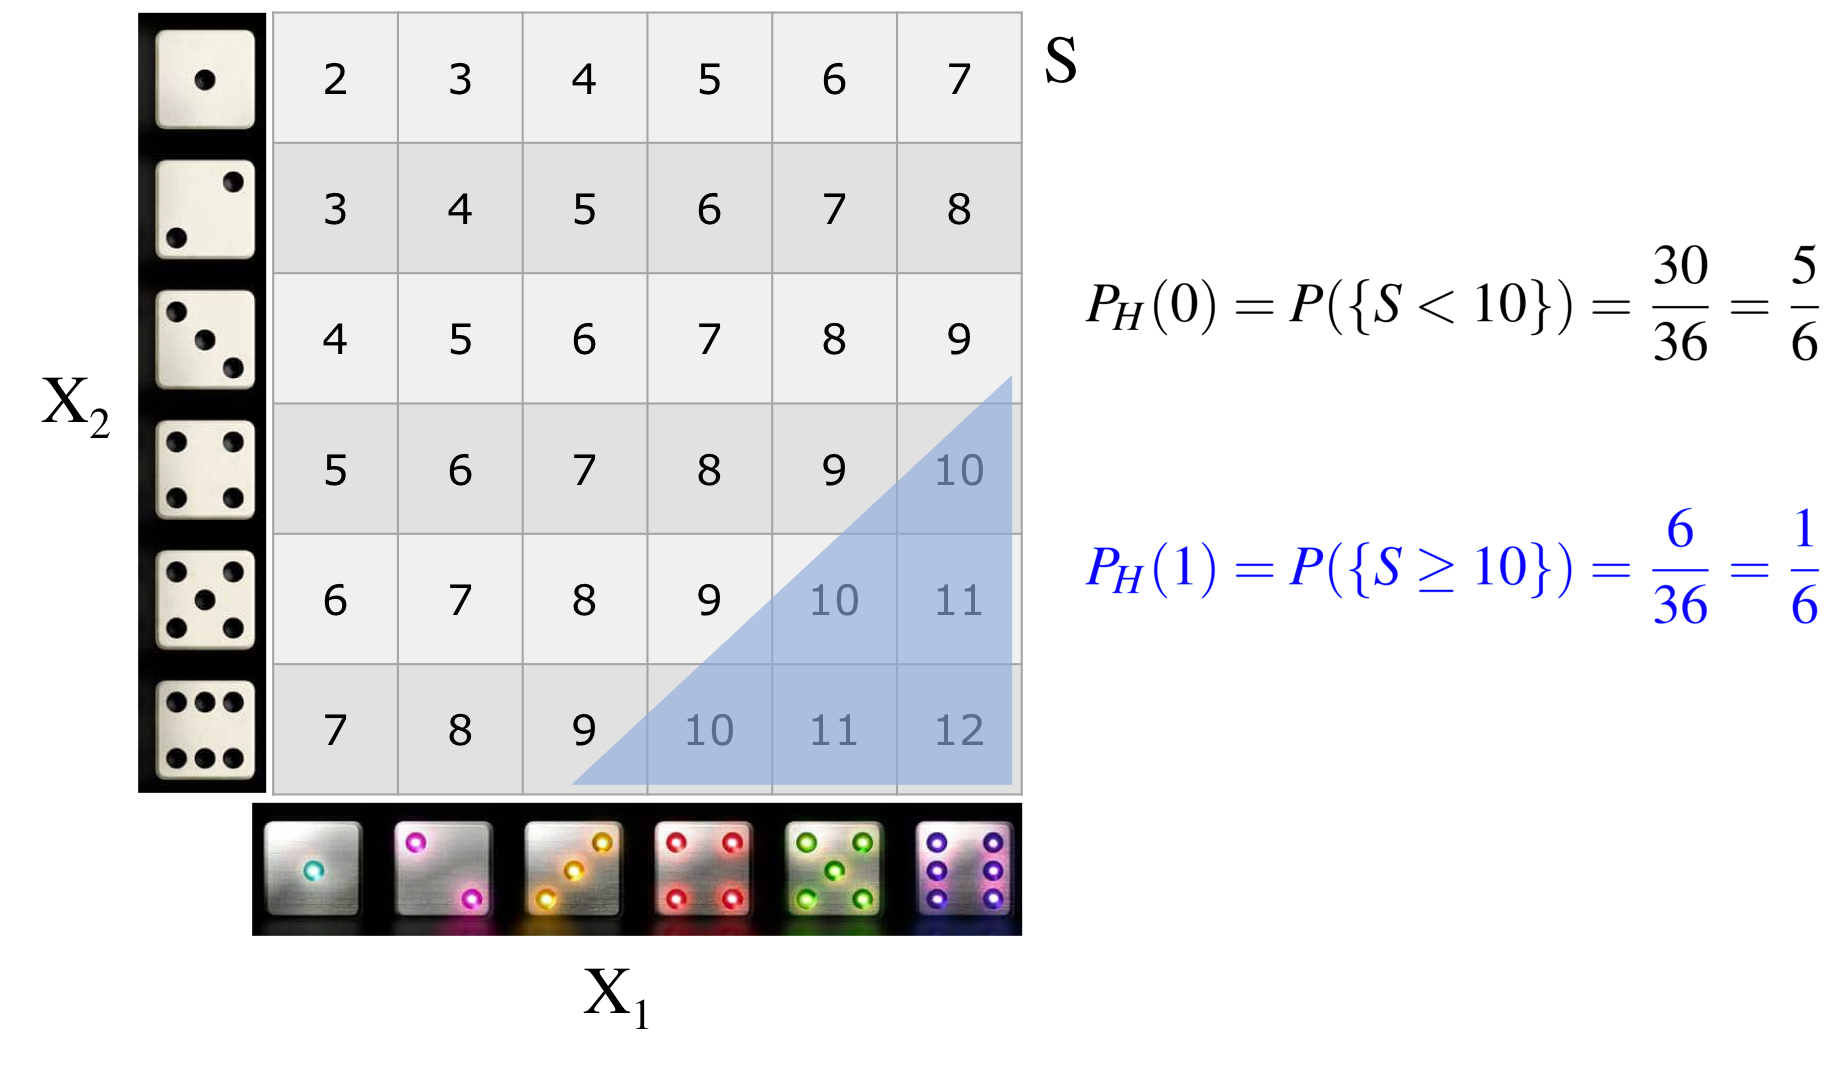
\includegraphics[width=10cm]{Figures/Dice.png}
        \end{center}
        \caption{All combinations of of $X_1$ and $X_2$ are equally probable, and therefore each of the $36$ results represented in the figure have a probability of $1/36$. Counting the number of occurrences of particular values of $S$ or $H$, the distribution of these variables can be calculated.\label{fig:dice}}
    \end{figure}
    
    Since we have to provide the criterion that minimizes the probability of error, we can then conclude that we should always decide in favor of hypothesis 0:
    $$d^\star = 0,$$
with a probability of error of  $1/6$.
    
    A final remark is in order. Note that the probability of error of each criterion is given by the {\em a priori} probability of the complementary hypothesis. This implies that, to minimize the probability of error, we have to decide in favor of the hypothesis with a larger {\em a priori} probability.

    \item[b)] In real applications, there are scenarios where not all the errors should be given the same importance. Here, we introduce the concept of {\em cost} to model the penalty that should be assigned to different kinds of errors.\footnote{In some cases rather than working with the minimization of a cost we might pursue the maximization of a profit. Both scenarios can be shown to be completely equivalent, but in this course we will always deal with cost functions.}
    
    Since different kinds of errors can be observed in different experiments, the cost can also be modeled with a random variable $C$. In this particular problem, $C$ can take four different values that we will denote as $c_{dh}$, for $d, h \in \{0,1\}$. That is, $c_{dh}$ is the cost of deciding $d$ when the true hypothesis was $h$. According to the wording, the costs are:
    \begin{equation*}
    c_{dh} = \left\{ \begin{array}{l}c_{00}=c_{11}= 0 \\ c_{01} = 1 \\ c_{10} = c\end{array}\right.    
    \end{equation*}
    
    Since $C$ is a function of $H$, it is also a random variable, for which its distribution could be obtained (from the probability distribution of $H$, $P_H(h)$). However, in this problem we only need to compute the expected cost of both detectors, that is,
    
    \begin{itemize}
        \item For the detector $d=0$:
        $$\widebar C = \mathbb{E}\{c_{dh}\} = \mathbb{E}\{c_{0h}\} = \sum_{h=0}^1 c_{0h} P_H(h) = c_{00}P_H(0) + c_{01}P_H(1) = \frac{1}{6}.$$
        \item For the detector $d=1$:
        $$\widebar C = \mathbb{E}\{c_{dh}\} = \mathbb{E}\{c_{1h}\} = \sum_{h=0}^1 c_{1h} P_H(h) = c_{10}P_H(0) + c_{11}P_H(1) = \frac{5 c}{6}.$$
    \end{itemize}

    \item[c)] To minimize the expected cost, we have to compare the costs that we calculated in the previous subsection
    $$\widebar C (d=0) \dunodcero \widebar C (d=1),$$
    which results in
    $$c \dceroduno \frac{1}{5}.$$
    
    Let us check, using our intuition, that this result makes sense. To start with, note that when the penalty given to wrongly deciding $d=1$ is unitary ($c_{10}=c=1$), both kinds of errors are identical. In such case, it can be seen that minimizing the expected cost is the same as minimizing the probability of error, and we should decide $d=0$ as in part a) of this problem. However, if $c_{10}$ is sufficiently small, deciding $d=1$ has a very small cost, so it can pay off to decide $d=1$ even though the number of errors is larger, as it will certainly be the case since hypothesis $H=0$ appears 5 times more often than hypothesis $H=1$. Hence, the expression above implies that if $c < 1/5$ then detector $d=1$ yields a smaller expected cost.
\end{itemize}
\end{solution}


\subsection{Example 2: Binary decision with observations}
\label{subsec:example2}

\begin{problem}
Consider now the scenario described in the previous example, with the difference that, before deciding in favor of one of the hypotheses, we are allowed to see the result of the first die, $X_1$. In this case, we will therefore be able to take a more informed decision since knowing such value carries information about the value of $S$.
\begin{itemize}
    \item [a)] Calculate the probability of error incurred by each possible decision ($d=0$ and $d=1$) for each value of $X_1$.
    \item [b)] Design the detector that minimizes the probability of error, and compute the probability of error of such detector.
    \item[c)] Obtain the test statistic that minimizes the cost described in the previous example, for the particular case $c=1/4$.
\end{itemize}
\end{problem}

\begin{solution}
The main difference of the scenario described in this problem with respect to that of the previous example is that, in this case, the detector can be a function of $X_1$. As a result, the decision may change from experiment to experiment, depending on the value of  $X_1$.

Precisely, when designing a detector our goal is to assign each possible value of the observations to a particular decision. In other words, if the same input is observed twice, the output must be the same in both cases, since the mapping from the observations to the decisions is assumed to be deterministic. We will say more on this later on, but for now, we focus on providing answers to the considered problem.

\begin{itemize}
    \item [a)] We will follow along the same lines of the previous exercise to compute the probability of error for the two possible decisions. Notice, however, that in this case we will be conditioning these probabilities on the value of $X_1$.
    \begin{itemize}
        \item For $x_1 \in \{1,2,3\}$, hypothesis $H=1$ can never hold. Therefore, in this case it seems obvious that deciding $d=0$ would guarantee a zero probability of error. More formally:
        $$\text{If } x_1 \in \{1,2,3\} \rightarrow \left\{\begin{array}{l} d=0 \rightarrow P_e = P(d\neq H|x_1\in \{1,2,3\}) = P_{H|X_1}(1|x_1\in \{1,2,3\}) = 0 \\ d=1 \rightarrow P_e = P(d\neq H|x_1\in \{1,2,3\}) = P_{H|X_1}(0|x_1\in \{1,2,3\}) = 1\end{array}\right.$$
        \item For $x_1 = 4$, there is only one possibility out of 6 that hypothesis $H=1$ is correct (for $x_2=6$). This allows us to easily compute the error of both criteria. Repeating this  for the remaining values of $X_1$, we obtain the following probabilities of error conditioned on $X_1$.
        $$\text{If } x_1 =4 \rightarrow \left\{\begin{array}{l} d=0 \rightarrow P_e = P(d\neq H|x_1=4) = P_{H|X_1}(1|x_1=4) = \frac{1}{6} \\ d=1 \rightarrow P_e = P(d\neq H|x_1=4) = P_{H|X_1}(0|x_1=4) = \frac{5}{6}\end{array}\right.$$
        $$\text{If } x_1 =5 \rightarrow \left\{\begin{array}{l} d=0 \rightarrow P_e = P(d\neq H|x_1=5) = P_{H|X_1}(1|x_1=5) = \frac{2}{6} = \frac{1}{3}\\ d=1 \rightarrow P_e = P(d\neq H|x_1=5) = P_{H|X_1}(0|x_1=5) = \frac{4}{6} = \frac{2}{3}\end{array}\right.$$
        $$\text{If } x_1 =6 \rightarrow \left\{\begin{array}{l} d=0 \rightarrow P_e = P(d\neq H|x_1=6) = P_{H|X_1}(1|x_1=6) = \frac{3}{6} =\frac{1}{2} \\ d=1 \rightarrow P_e = P(d\neq H|x_1=6) = P_{H|X_1}(0|x_1=6) = \frac{3}{6} = \frac{1}{2}\end{array}\right.$$
    \end{itemize}
In this case, the probability of error associated to each decision is given by the probability of the complementary hypothesis. The difference is that now we have to use {\em a posteriori} probabilities of the hypotheses, given that the decision is taken using some information (the value of $X_1$), and this knowledge refines how likely we can expect the different hypotheses to be. Figure \ref{fig:posteriorprobs} depicts these probabilities. Note that to compute the probability conditioned on each value of $X_1$, we need to consider only the values of $S$ that are associated to the corresponding column.
    
    \begin{figure}
        \begin{center}
            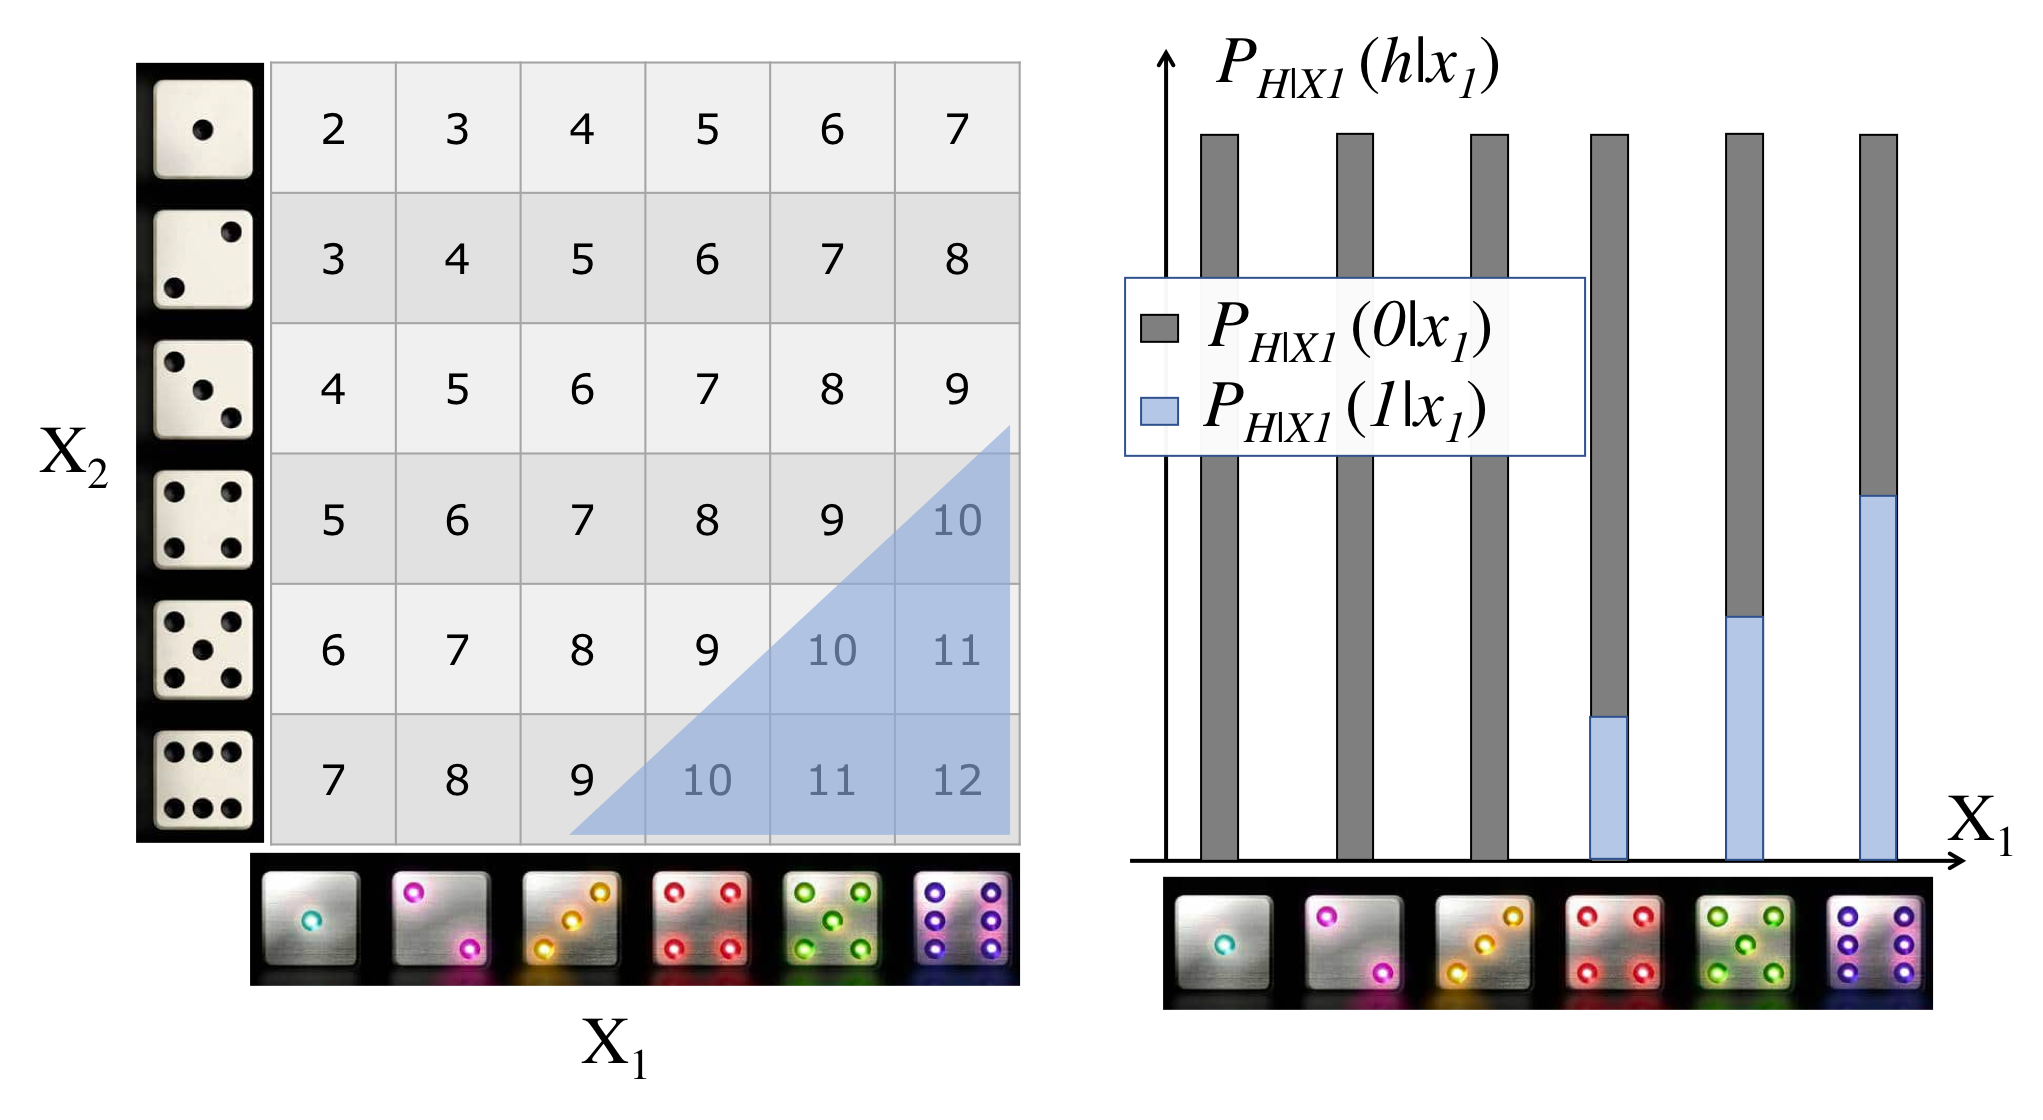
\includegraphics[width=10cm]{Figures/Dice_posterior.png}
        \end{center}
        \caption{To calculate posterior probabilities of the hypothesis, we need to count how many results in each column correspond to hypothesis 0 and how many correspond to hypothesis 1. Note that $P_{H|X_1}(0|x_1) + P_{H|X_1}(1|x_1) = 1$ for all values of $X_1$.\label{fig:posteriorprobs}}
    \end{figure}

    \item[b)] To minimize the probability of error of the detector, it suffices to minimize the conditional probability of error. In this case, since the decision becomes a function of $X_1$, $D = f(X_1)$, the detector becomes a random variable itself. Designing the detector consists in obtaining such function $f(\cdot)$. In this course, we only consider that $f(\cdot)$ is deterministic, i.e., if the same $x_1$ is observed twice the detector will produce the same output in both cases. This implies that we can alternatively interpret the goal of designing a detector as partitioning the observation space into as many regions as the number of hypotheses.
    
    Using the results from the previous section, it follows that, to minimize the error at every point, we need to select the hypothesis with the largest {\em a posteriori} probability, i.e., the test statistic that results in a minimum probability of error is:
    $$d(x_1) =\arg\max_i P_{H|X_1}(i|x_1).$$
    This expression gives the name to the detection criterion, is known as the {\em Maximum a Posteriori} (MAP) detector. Actually, maximizing the {\em a posteriori} probability is the criterion that minimizes the probability of error in general. 
    
    Since $P_{H|X_1}(0|x_1=6) = P_{H|X_1}(1|x_1=6)$, for $x_1 = 6$ deciding in favor of either hypotheses results in the same probability of error ($1/2$). For the remaining values, $d=0$ should be selected. Finally, using the law of total probability, the probability of error becomes
    \begin{align}P_e = P(D\neq H) & = \sum_{x_1=1}^6 P(D\neq H| x_1) P_{X_1}(x_1) \nonumber \\
    & = P(D\neq H| x_1=1) P_{X_1}(1) + P(D\neq H| x_1=2) P_{X_1}(2) \nonumber \\
    & \;\;\;\;\;\;+ P(D\neq H| x_1=3) P_{X_1}(3) + P(D\neq H| x_1=4) P_{X_1}(4) \nonumber \\
    & \;\;\;\;\;\;+ P(D\neq H| x_1=5) P_{X_1}(5) + P(D\neq H| x_1=6) P_{X_1}(6) \nonumber \\
    & = \frac{1}{6} \left[0 + 0 + 0 + \frac{1}{6} + \frac{1}{3} + \frac{1}{2}\right] = \frac{1}{6}.\nonumber
    \end{align}
    
    \item[c)] In this part of the problem we need to minimize the expected cost. Similarly to what we did for the probability of error, we will first compute the expected cost associated to every decision and observation $x_1$, and then at each point we will simply select the decision criterion that incurs in a minimum expected cost.
    
    $$\text{If } x_1 \in \{1,2,3\} \rightarrow \left\{\begin{array}{l} d=0 \rightarrow \mathbb{E}\{C_{0H}|x_1\in \{1,2,3\}\} = 0 \\ d=1 \rightarrow \mathbb{E}\{C_{1H}|x_1\in \{1,2,3\}\} = c_{10} P_{H|X_1}(0|x_1\in \{1,2,3\}) = c_{10} = \frac{1}{4}\end{array}\right.$$
    $$\text{If } x_1 =4 \rightarrow \left\{\begin{array}{l} d=0 \rightarrow \mathbb{E}\{C_{0H}|x_1=4)\} = c_{01} P_{H|X_1}(1|x_1=4) = \frac{1}{6} \\ d=1 \rightarrow \mathbb{E}\{C_{1H}|x_1=4)\} = c_{10} P_{H|X_1}(0|x_1=4) = \frac{5}{24}\end{array}\right.$$
    $$\text{If } x_1 =5 \rightarrow \left\{\begin{array}{l} d=0 \rightarrow \mathbb{E}\{C_{0H}|x_1=5)\} = c_{01} P_{H|X_1}(1|x_1=5) = \frac{2}{6} \\ d=1 \rightarrow \mathbb{E}\{C_{1H}|x_1=5)\} = c_{10} P_{H|X_1}(0|x_1=5) = \frac{1}{6}\end{array}\right.$$
    $$\text{If } x_1 =6 \rightarrow \left\{\begin{array}{l} d=0 \rightarrow \mathbb{E}\{C_{0H}|x_1=6)\} = c_{01} P_{H|X_1}(1|x_1=6) = \frac{1}{2} \\ d=1 \rightarrow \mathbb{E}\{C_{1H}|x_1=6)\} = c_{10} P_{H|X_1}(0|x_1=6) = \frac{1}{8}\end{array}\right.$$
    
    Then, the detector that minimizes the expected cost is
%    \begin{equation}
  %      
   % \end{equation}
   \begin{equation*}
   d^\star = \begin{cases}  0, & \text{if } X_1 \in \{1,2,3,4\}, \\ 1, & \text{if } X_1 \in \{5, 6\},
   \end{cases}
   \end{equation*}
    with the expected cost given by
    \begin{align*}
        \mathbb{E}\{C\} & = \sum_{x_1=1}^6 \mathbb{E}\{C | x_1\} P_{X_1}(x_1) \\ &= \frac{1}{6}[0+ 0 +0 + \frac{1}{6} + \frac{1}{6} + \frac{1}{8}] \\ &= \frac{11}{6\cdot 24},
    \end{align*}
    which follows from the law of total probability. One final comment is in order. Using a detector that exploits the value of an observation variable, we were able to reduce the expected cost with respect to the value obtained in the first example.
    
\end{itemize}

\end{solution}

So far, we have learned that the {\em a posteriori} probability of $H$ given the observations plays a key role in detection problems. In the first two examples, obtaining such probability was rather straightforward given the inherent mechanism for the generation of the hypotheses: observations take place first, and the hypothesis depends directly on these observations. Now, we will consider the case in which the generation of the hypothesis occurs first, and then observations are drawn according to their probability distribution given the hypothesis. This scenario is frequently encountered in many real problems. When this is the case, one can more easily get access to the {\em likelihoods} of each hypothesis, and the {\em a posteriori} probabilities need to be evaluated exploiting Bayes' Theorem.

\subsection{Example 3: Working the solution from the likelihoods}
\label{subsec:example3}

\begin{problem}
	Consider now a new game that involves two coins, one of them is fair whereas for the second one, the probability of heads doubles the probability of tails. In this game, a coin is first selected, and the goal is to guess which is the selected coin using as observations the result of flipping the coin $n$ times. Therefore, this problem can also be seen as a hypothesis testing problem, where one has to decide whether the selected coin was the fair one (hypothesis $H=0$) or the loaded one (hypothesis $H=1$).
	
	\begin{itemize}
		\item [a)] Without assuming any other information, design a detector for the aforementioned hypothesis test.
		\item [b)] Discuss how you would design a detector that minimizes the probability of error, and what additional information you would need for that.
	\end{itemize}
\end{problem}

\begin{solution}
	
	We denote by $\bf X$ the vector that  contains all the available observations to take the decision, i.e., the result of each coin flipping: ${\bf X} = (X^{(1)}, X^{(2)}, \ldots, X^{(n)})^\top$. Each of these variables can be a head or a tail: $X^{(i)} \in \left\{\circ,\times \right\}$. We will denote by $n_\circ$ and $n_\times$ the number of observed heads and tails, respectively. Obviously, we have $n = n_\circ + n_\times$.
	
	\begin{itemize}
		\item [a)] The only statistical information available in this section is the probability of observing a head or a tail for both hypotheses:
		\begin{align*}
		P_{X^{(i)}|H}(\circ | 0) &= \frac{1}{2}, & P_{X^{(i)}|H}(\times | 0) &= \frac{1}{2},
		\end{align*}
		and
		\begin{align*}
		P_{X^{(i)}|H}(\circ | 1) &= \frac{2}{3}, & P_{X^{(i)}|H}(\times | 1) &= \frac{1}{3}.
		\end{align*}
		Now, since there are available $n$ observations, we can also compute the joint probability of the observation vector $\bf X$:
		\begin{align*}
		P_{{\bf X}|H}({\bf x}|0) &= \left( \frac{1}{2}\right)^{n}, & P_{{\bf X}|H}({\bf x}|1) &= \left( \frac{2}{3}\right)^{n_\circ} \left( \frac{1}{3}\right)^{n_\times}.
		\end{align*}		
		These two expressions above are the joint probabilities of all observed variables given the hypothesis, and are usually referred to as the likelihoods of hypothesis $0$ and $1$. Essentially, the likelihoods express how well the observed data can be explained by each of the hypotheses.
		
		When the only available information is the likelihoods, a reasonable approach to follow is deciding in favor of the hypothesis that maximizes the likelihood. For this example, the so-called {\em maximum likelihood} (ML) detector is given by
		$$P_{{\bf X}|H}({\bf x}|0)\dceroduno P_{{\bf X}|H}({\bf x}|1) \Rightarrow \left( \frac{1}{2}\right)^{n} \dceroduno \left( \frac{2}{3}\right)^{n_\circ} \left( \frac{1}{3}\right)^{n_\times}.$$
		A convenient way to simplify this expression consists in taking logarithms on both sides of the inequality. Note that, in order to take logarithms, we need to make sure that the arguments thereof are strictly positive, which holds for both sides of the equation above. Then, taking logarithms and simplifying the resulting expression yields
		$$(n_\circ + n_\times) \log\frac{1}{2} \dceroduno n_\circ \log\frac{2}{3} + n_\times \log\frac{1}{3},$$
		or, equivalently,
		$$\frac{n_\times}{n_\circ} \dceroduno \frac{\log\frac{2}{3} - \log\frac{1}{2}}{\log\frac{1}{2} - \log\frac{1}{3}}.$$
		This equation translates into a partition of the observation space. In fact, we see that the detector does not depend on the value of particular observations, but just on the total number of heads and tails (i.e., the order in which the coin flippings are observed does not matter). Moreover, it also implies that a larger number of observed heads favors the decision $D=1$, which aligns with the fact that the probability of heads is larger than the probability of tails when $H=1$.
		
		\item[b)] Now, we need to study the minimization of the probability of error, defined as
		$$P_e = P(D\neq H) = \sum_{\bf x} P(d\neq H | {\bf X}={\bf x}) P_{\bf X}({\bf x}).$$
		In order to grasp the meaning of $P_e$, we need to emphasize that for any particular detector, there is a deterministic relation between $D$ and ${\bf X}$. Since the probability of error for a given observation vector is $P(d\neq H | {\bf X}={\bf x})$, the expectation of this value needs to be taken with respect to ${\bf X}$ to obtain the probability of error. The minimization of $P_e$ is equivalent to the minimization of each element in the above summation. That is, for each possible observation vector ${\bf x}$ we need to take the decision that minimizes the probability of error for that particular value of ${\bf x}$. Since there are only two hypothesis, the probability of incurring in an error if we decide in favor of one of the hypothesis is the probability of the non-selected hypothesis, i.e.,
		$$\text{If we decide } d=0 \qquad \rightarrow \qquad  P(H \neq 0 | {\bf X}={\bf x}) = P_{H|{\bf X}}(1|{\bf x}),$$
		$$\text{If we decide } d=1 \qquad \rightarrow \qquad  P(H\neq 1 | {\bf X}={\bf x}) = P_{H|{\bf X}}(0|{\bf x}).$$
		Therefore, in order to minimize the probability of error at each ${\bf x}$, and therefore to minimize the overall probability of error, we need to follow the criterion:
		$$P_{H|{\bf X}}(1|{\bf x}) \dunodcero P_{H|{\bf X}}(0|{\bf x}),$$
		which is, as described above, the {\em Maximum a posteriori} (MAP) detector. In other words, maximizing the likelihood does not necessarily minimize the probability of error, which is actually minimized by maximizing the {\em a posteriori} probabilities of each hypotheses. This makes sense, since the likelihood just measures how well the observations fit with a given hypothesis, but ignores the {\em a priori} probability of the hypotheses. Then, we can  decide in favor of a hypotheses with smaller likelihood if its {\em a priori} probability is sufficiently larger than the probability of the other hypothesis. This can be explicitly quantified by means of Bayes' Theorem, which states that
		$$P_{H|{\bf X}}(h|{\bf x}) = \frac{P_{{\bf X}|H}({\bf x}|h) P_{H}(h)}{P_{\bf X}({\bf x})}.$$
		Bayes' Theorem shows that the maximization of  the {\em a posteriori} probability of each hypothesis (and therefore to minimize the probability of error) requires taking into account both the likelihoods and the {\em a priori} probabilities of the hypotheses.
		
		In summary, in order to design a detector (or classifier) that minimizes the probability of error, we would need to know the {\em a priori} probability of each hypothesis. Moreover, if the goal were to minimize a cost function, we would still need to rely on {\em a posteriori} probabilities.
		
	\end{itemize}
	
\end{solution}

In the previous examples, we have introduced a number of important concepts in detection problems: hypotheses, {\em a priori} and {\em a posteriori} probability, likelihood, probability of error, and (expected) cost. We have also learned that, for the design of detectors when there are available observations, the distribution that provides {\bf  the most valuable information is the {\em a posteriori} distribution of the hypotheses given such observations}. If this distribution is available, we can compute the performance of {\bf any} detector in terms of its probability of error or expected cost (performance analysis problems). Based on these performance metrics, we can also design detectors that minimize each criterion (design problem). 

%\begin{problem}
%    Transmission of a binary symbol over a Gaussian channel (TBD).
% \end{problem}